\documentclass{acm_proc_article-sp}
\usepackage{tikz}
\usepackage{multicol}
\usepackage{url}
\usepackage[shortlabels]{enumitem}
\usepackage{fontspec}
\usetikzlibrary{plotmarks}
\begin{document}
\title{Algorithm and Data Structure Coursework: \\K-Means Feature for
Image Retrieval}
\subtitle{}
%
\numberofauthors{2} %  in this sample file, there are a *total*
% of EIGHT authors. SIX appear on the 'first-page' (for formatting
% reasons) and the remaining two appear in the \additionalauthors section.
%
\author{\alignauthor{Qiwei Feng}\\
       \affaddr{2011011250, IIIS-10}\\
       \affaddr{Tsinghua University}\\
       \email{gdfqw93@163.com}
   \alignauthor{Pufan He}\\
       \affaddr{2011011307, IIIS-10}\\
       \affaddr{Tsinghua University}\\
       \email{hpfdf@126.com}
}
\date{16 June 2015}

\maketitle
\begin{abstract}
        This project implements a similar image search algorithm (image
        retrieval) based on multiclass classification and K-Means feature. Our
        training phase includes image resizing, image patch extraction, patch
        sampling, PCA whitening, K-Means for patches, feature extraction and
        multiclass SVM\@. We use 218-dimension K-Means and RGB, HSV color moment.
        The training phase takes no greater than one hour in time, 8GB in memory.
        Finally we obtained 69.82\% accuracy on test data classification.

We have made our work open, and the full project codes can be found at
\texttt{https://github.com/caiwaifung/lastcourse}.
\end{abstract}

\keywords{Image Retrieval, Image Classification, SVM, Whitening, K-Means}

%------------------------------------------------------------------------%
\section{Introduction}
% say what we want to do, want we did, how well we could make
% briefly discuss how we did: the main part is in "Implementation" section

%------------------------------------------------------------------------%
\section{Implementation}
% say how we implementation the system
We built a system to extracting features from images as well as
    training model and answering queries of finding related images.
The whole system is written in MATLAB\@.

The system contains feature extracting part and SVM training and testing part.
In the feature extracting part,
    we use both features from K-Means method~\cite{coates2011analysis},
    and the RGB and HSV color moments.
We use 200-dimension K-Means features and 18-dimension color moment
features (9 for RGB and 9 for HSV).
The K-Means method contains patch extracting, patch whitening,
    patch sampling and K-Means clustering,
    and feature extrating.
The color moment method makes use of 3 common color moments for 
    each channel of RGB and HSV colors.
At last, we put the features into SVM and make the classification possible.
The related image search process is done by simply finding
    the closest feature in the same catelogy.

The following subsections includes the details of our algorithms.

\subsection{Patch Extracting and Sampling}

The key idea of K-Means featuring is to find the most common
    patches in all images, and build features based on that
    common patches (called centroids).
Let $w$ be the size of the centroids (set to $6$ in our implementation).
For an $l$-by-$m$ image,
we will consider all its sub-images (patches) of size $w$-by-$w$;
there are totally $(l-w+1)(m-w+1)$ such patches.
Each patch can be represented into a vector of length $3w^2 = p$,
    so one image can be represented into a $n$-by-$p$ matrix,
    where $n=(l-w+1)(m-w+1)$.
We represent all images into this matrix form.
This process is called \emph{patch extracting}.

We need a large amount of sampling patches for the K-Means clustering process.
We simply random selected $t\approx 1000000$ patches
    from all the images' matrices.
The sampled patches is a matrix $P$ of size $t$-by-$p$.

\subsection{Whitening}

Directly compute the square distance between two $6\times 6\times 3$ patches is not
very reasonable. We use the idea of whitening from \cite{coates2011analysis} to
transform our patches into normalized $108$-length real vector, so that when
consider the transformed patch as a random variable, the mean of every entry
is $0$ and the variance of every entry is $1$. Whitening could reduce possible
bias in patch component, and returns more robust K-Means result.

This can be done by a PCA transform:
\begin{equation}
        X_{\text{wh}}=\text{diag}\left(1/\sqrt{\text{diag}(S)+\epsilon}\right)\times U^T
        \times (X-\mu),
\end{equation}
where the covariance matrix SVD decomposite into $U,S,V$, and $\mu$ is the mean
$X$. We use the built-in SVD function in matlab to achieve high efficiency.

\subsection{K-Means Clustering}

We want $k=200$ centroids of all sampled patches.
We do the K-Means clustering for those patches,
    and take the final $k$ ``means''.
The final centroids can be represented by a matrix $C$ of size $k$-by-$p$.

%TODO more

\begin{center}
        Without Whitening
        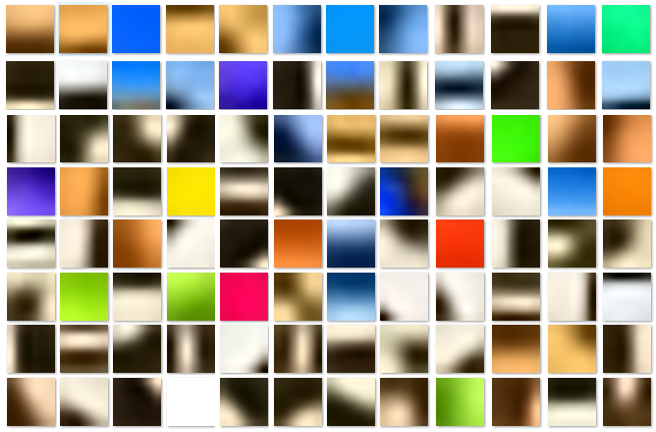
\includegraphics[width=0.8\linewidth]{004.png}

        With Whitening
        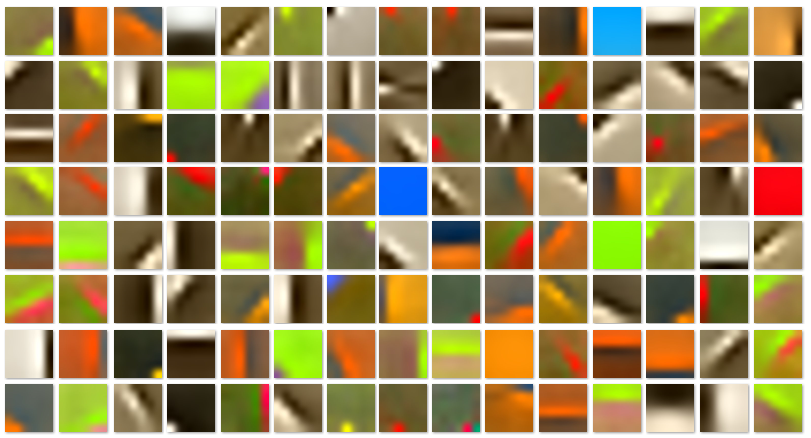
\includegraphics[width=0.8\linewidth]{005.png}
\end{center}

\subsection{Feature Extracting}

Now consider an $l$-by-$m$ image.
We know that it has $n$ patches, so it's an matrix $G$ of size $n$-by-$p$.
We first calculate the distance between each patch
and each centroids, resulting in a distance matrix $D\in\mathbb{R}^{n\times k}$
where $D_{ij}$ is the distance from the $i$-th patch
and the $j$-th centroid.
Then, we normalize each row of $D$ by
    subtracting its mean and dividing its standard variance.
We negate each elements of the normalized $D$, elimate
    all negative elements by setting them to zeros,
    and get the new matrix $D^*$.
Here, $D^*_{ij}$ being large means that the $i$-th patch
    looks close to the $j$-th centroid.

Finally, we sum up all rows and get a $k$-dimension feature for this image.

\subsection{Color Moment}

For each color channel, the three color moments is defined as following:
\begin{itemize}
    \item The first is the mean of all pixels.
    \item The second is the standard deviation, that is:
        \[
            \sqrt{\frac{1}{N} \sum_{i=1}^N {(a_i-E[a])}^2}.
        \]
    \item The second is the skewness, that is:
        \[
            \sqrt[3]{\frac{1}{N} \sum_{i=1}^N {(a_i-E[a])}^3}.
        \]
\end{itemize}

\subsection{Multiclass SVM}

\subsection{Related Image Search}

After classification for a query image,
    we simply find the closest features in the same catelogy,
    and output the corresponding images as the related results.

Note that a trick can be used to calculate the distance
between each row of a matrix $A\in\mathbb{R}^{n*k}$ 
and a matrix $B\in\mathbb{R}^{m*k}$.
We want $C$ where $C_{ij}=||A_i - B_j||$. Have
\begin{align*}
    C_{ij} &= \sum_x {(A_{ix} - B_{jx})}^2 \\
           &= \sum_x A_{ix}^2 + \sum_x B_{jx}^2 - 2 \sum_x A_{ix} B_{jx} \\
           &= X_i + Y_j - 2 Z_{ij}.
\end{align*}
Here, $X$ and $Y$ are easy to calculate.
$Z=AB^T$ can be fastly calculated using MATLAB (because MATLAB uses MKL
internally).
Thus the distance can be computed within a short period of time,
    which gives us no reason to
    use any advanced data structure
    to find the closest images.

%------------------------------------------------------------------------%
\section{Experiments}

\subsection{Data Set}
Class labels $1\leq C \leq 10$:
\begin{enumerate}[1.]
\item Bird.
\item Insect.
\item Butterfly.
\item Waterwheel.
\item Construction.
\item Piano.
\item Airplane.
\item Wine.
\item Woman.
\item Flower.
\end{enumerate}

\subsection{Without Whitening}

\subsection{With Whitening}

\subsection{Final Test}

The distribution of predicted labels:
\begin{multicols}{2}\tiny\tiny
\begin{verbatim}
1-1: 41 |################ 71.93 %
1-2:  3 |#
1-3:  1 |
1-4:  3 |#
1-5:  0 |
1-6:  1 |
1-7:  2 |
1-8:  2 |
1-9:  1 |
1-10: 3 |#

2-1:  7 |##
2-2: 28 |########### 49.12 %
2-3:  8 |###
2-4:  1 |
2-5:  0 |
2-6:  0 |
2-7:  2 |
2-8:  4 |#
2-9:  3 |#
2-10: 4 |#

3-1:  0 |
3-2:  5 |##
3-3: 46 |################## 85.19 %
3-4:  1 |
3-5:  0 |
3-6:  1 |
3-7:  0 |
3-8:  0 |
3-9:  1 |
3-10: 0 |

4-1:  0 |
4-2:  1 |
4-3:  3 |#
4-4: 38 |############### 73.08 %
4-5:  4 |#
4-6:  2 |
4-7:  0 |
4-8:  2 |
4-9:  2 |
4-10: 0 |

5-1:  0 |
5-2:  0 |
5-3:  0 |
5-4:  7 |##
5-5: 40 |################ 68.97 %
5-6:  2 |
5-7:  1 |
5-8:  5 |##
5-9:  3 |#
5-10: 0 |

6-1:  1 |
6-2:  2 |
6-3:  0 |
6-4:  6 |##
6-5:  1 |
6-6: 38 |############### 58.46 %
6-7:  0 |
6-8:  7 |##
6-9: 10 |####
6-10: 0 |

7-1:  3 |#
7-2:  1 |
7-3:  1 |
7-4:  1 |
7-5:  1 |
7-6:  2 |
7-7: 43 |################# 81.13 %
7-8:  0 |
7-9:  0 |
7-10: 1 |

8-1:  2 |
8-2:  1 |
8-3:  0 |
8-4:  2 |
8-5:  5 |##
8-6:  4 |#
8-7:  0 |
8-8: 53 |##################### 74.65 %
8-9:  3 |#
8-10: 1 |

9-1:  3 |#
9-2:  1 |
9-3:  0 |
9-4:  0 |
9-5:  0 |
9-6:  5 |##
9-7:  1 |
9-8:  4 |#
9-9: 35 |############## 71.43 %
9-10: 0 |

10-1: 3 |#
10-2: 7 |##
10-3: 2 |
10-4: 4 |#
10-5: 1 |
10-6: 1 |
10-7: 1 |
10-8: 5 |##
10-9: 7 |##
10-10:66|########################## 68.04 %
\end{verbatim}
\end{multicols}
Final Accuracy of 10-classification:
\begin{verbatim}
Accuracy = 69.8206% (428/613) (classification)
\end{verbatim}

On training set:
\begin{verbatim}
Accuracy = 88.96% (4448/5000) (classification)
\end{verbatim}
\begin{center}
Query image | 3 closest images in predicted class
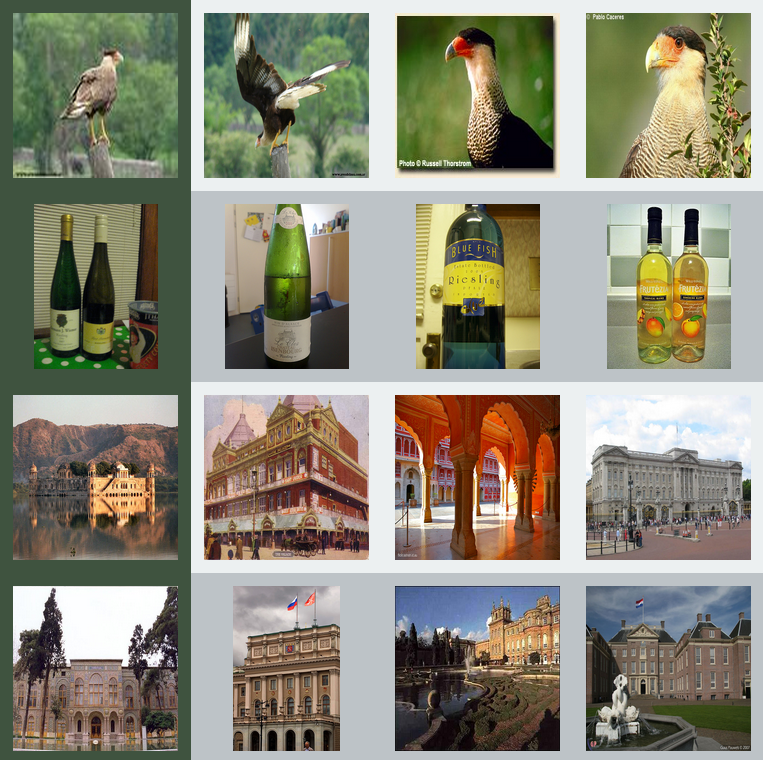
\includegraphics[width=0.7\linewidth]{001.png}\\
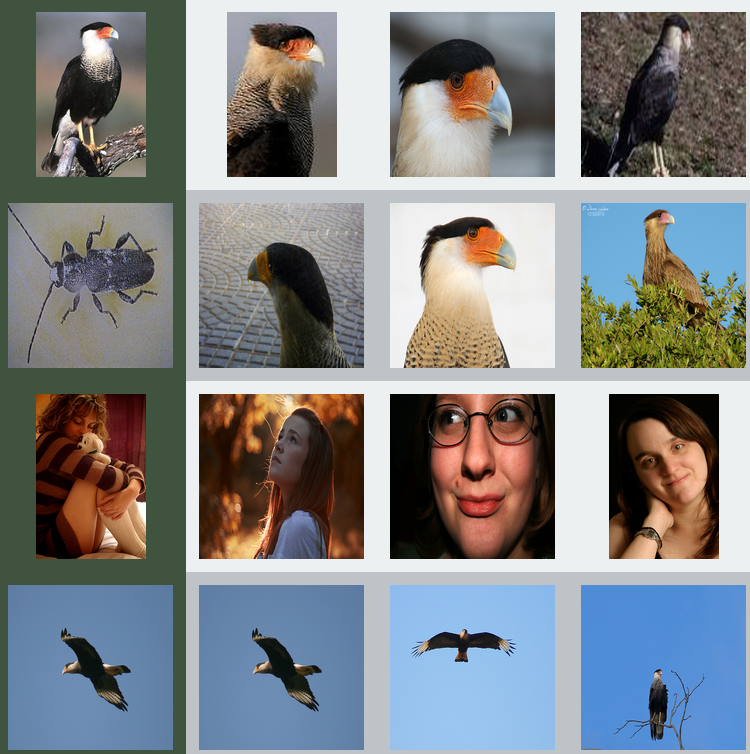
\includegraphics[width=0.7\linewidth]{002.png}\\
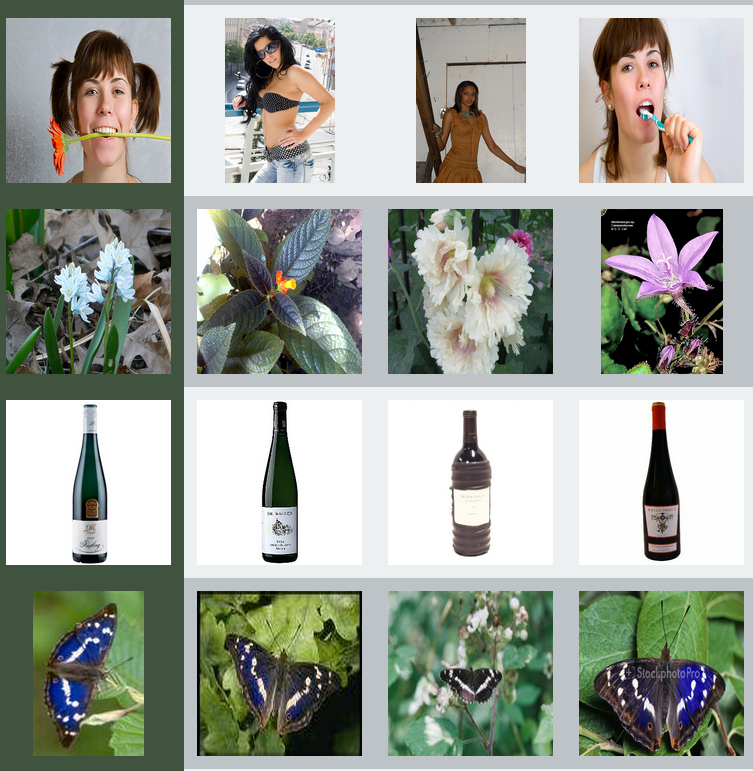
\includegraphics[width=0.7\linewidth]{003.png}
\end{center}

Please see \texttt{a.html} under \texttt{result.zip} for a more detailed demo.
%------------------------------------------------------------------------%
\section{Conclusion and Future Work}
We have implemented a full workflow of image retrieval problem. Our program is
integrated in one matlab module, and almost all parameters can be adjusted. We
implemented our own K-Means algorithm, and visualized our K-Means result on
patch clustering into $K$ images. The centroids we got prove to meet clear
patterns, which is similar to other successful convolutionary computer vision
systems. Our training phase and feature extraction process are highly
optimized, so that training 5000 images takes less than one hour, and
classifying 2000 test images takes less than one minutes. Our final accuracy
rate 69.82\% is also competitive in all current image 10-classification
algorithms using the same level of computing resources. The closest retrieval
demo brings very reasonable results as well.

However there are still many wrong predictions that are trivial for human. If
we use deeper machine learning model such as CNN, we may further improve our
accuracy. We can also generate small noises, random rotation, flipping, and
many other tricks to enrich the dataset for larger machine learning framework.
So if time permitting, we will try those algorithms.

%------------------------------------------------------------------------%
\nocite{*}
\bibliographystyle{abbrv}
\bibliography{sigproc} 

\balancecolumns{}

\end{document}
